\begin{center}
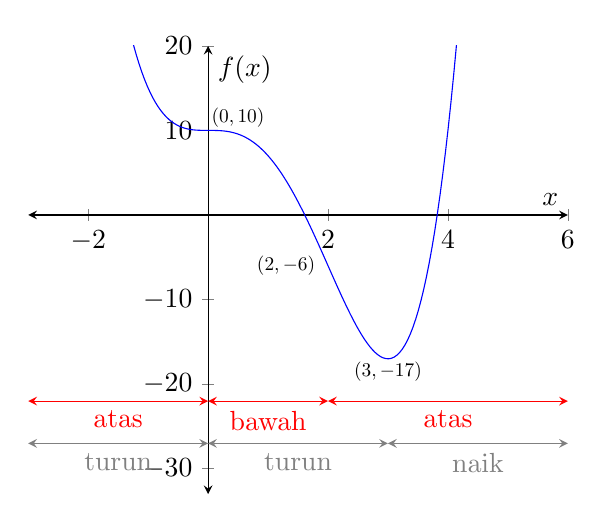
\begin{tikzpicture}[>=stealth]
\begin{axis}[
    xmin=-3,xmax=6,
    ymin=-33,ymax=20,
    axis x line=middle,
    axis y line=middle,
    axis line style=<->,
    xlabel={$x$},
    ylabel={$f(x)$},
    ]
    
    \addplot[no marks,blue, -] 
        expression[domain=-4:5,samples=200]{x^4-4*x^3+10};
    
    \point{blue}{(3,-17)};
    \node at (3,-18.5){\scalebox{0.7}{$(3,-17)$}};
    \point{blue}{(2,-6)};
    \node at (1.3,-6){\scalebox{0.7}{$(2,-6)$}};
    \point{blue}{(0,10)};
    \node at (0.5,11.5){\scalebox{0.7}{$(0,10)$}};
    
    \draw[red, <->] (-3,-22) -- node[below](){atas} (0,-22);
    \draw[red, <->] (0,-22) -- node[below](){bawah} (2,-22);
    \draw[red, <->] (2,-22) -- node[below](){atas} (6,-22);
    \draw[gray, <->] (-3,-27) -- node[below](){turun} (0,-27);
    \draw[gray, <->] (0,-27) -- node[below](){turun} (3,-27);
    \draw[gray, <->] (3,-27) -- node[below](){naik} (6,-27);
\end{axis}
\end{tikzpicture}
\end{center}